\documentclass[journal]{IEEEtran}
\usepackage{amsmath,amsfonts,amssymb}
\usepackage{algorithmic}
\usepackage{algorithm}
\usepackage{array}
\usepackage[caption=false,font=normalsize,labelfont=sf,textfont=sf]{subfig}
\usepackage{textcomp}
\usepackage{stfloats}
\usepackage{url}
\usepackage{verbatim}
\usepackage{graphicx}
\usepackage{cite}
\usepackage{booktabs}
\usepackage{multirow}
\usepackage{hyperref}

\hyphenation{op-tical net-works semi-conduc-tor IEEE-Xplore stegan-alysis}

\begin{document}

\title{Sudarshana: A Multi-Domain, Open-Set Steganalysis Framework with Cross-Attention Fusion and Verifiable Explainability}

\author{Mridul~B.,~\IEEEmembership{Student Member,~IEEE,}
        Research~Advisory~Board,~\IEEEmembership{Senior Member,~IEEE}
\thanks{This work was conducted as part of the Engineering Design and Innovation (EDI) initiative at Vishwakarma Institute of Technology (VIT), Pune, India.}
\thanks{M. B. is with the Department of Computer Engineering, Vishwakarma Institute of Technology, Pune 411037, India (e-mail: mridul@vit.edu).}}

\markboth{IEEE Transactions on Information Forensics and Security,~Vol.~XX, No.~Y, 2026}%
{B. \MakeLowercase{\textit{et al.}}: Sudarshana: Multi-Domain Open-Set Steganalysis Framework}

\maketitle

\begin{abstract}
As steganographic embedding paradigms evolve from classical spatial modifications to complex transform-domain perturbations and generative synthetic payloads, modern deep-learning steganalysts exhibit critical domain-myopia, cover-source sensitivity, and closed-set vulnerabilities. Existing state-of-the-art detectors (e.g., SRNet, Xu-Net, Yedroudj-Net) rely predominantly on spatial high-pass residuals, collapsing when tested across mismatched JPEG qualities, unseen embedding algorithms, or benign sensor noise. In this paper, we propose \textbf{Sudarshana} (StegShield), a multi-branch information forensics framework designed for robust cross-domain detection, open-set rejection, and verifiable attribution on edge hardware. Sudarshana integrates four complementary analysis pipelines: (i) spatial noise residual learning via 30 frozen Spatial Rich Model (SRM) filters, (ii) block Discrete Cosine Transform (DCT) frequency modeling, (iii) high-order statistical moment and histogram RS-analysis, and (iv) depthwise-separable generative artifact detection. These diverse representations are unified through a Transformer-based Cross-Attention fusion module that dynamically contextualizes inter-domain dependencies. To overcome closed-set overconfidence, we introduce a Helmholtz free-energy rejection engine that identifies out-of-distribution (OOD) stego algorithms and corrupted covers without retraining. Furthermore, we audit attribution veracity via a rigorous Grad-CAM faithfulness pipeline measuring pixel-level Intersection-over-Union (IoU) against exact bit-modification ground truths and progressive deletion drops. Finally, we demonstrate edge deployability via 8-bit dynamic integer quantization (INT8), achieving an $18.4\times$ memory reduction (from 21.31\,MB to 1.16\,MB) with 246.7\,ms inference on commodity edge processors.
\end{abstract}

\begin{IEEEkeywords}
Steganalysis, multi-domain fusion, cross-attention transformer, open-set recognition, energy-based OOD detection, explanation faithfulness, INT8 quantization.
\end{IEEEkeywords}

\section{Introduction}
\IEEEPARstart{I}{mage} steganography constitutes a major vector for clandestine data exfiltration and covert command-and-control operations across contested networks. While historical methods relied on deterministic Least Significant Bit (LSB) substitution in the spatial domain, contemporary steganographic techniques leverage adaptive content-adaptive distortion functions (e.g., WOW~\cite{holub2012designing}, S-UNIWARD~\cite{holub2014designing}, HILL~\cite{li2014new}) and transform-domain uniform embedding schemes (e.g., UERD~\cite{guo2014using}). Most recently, generative AI models (GANs, Invertible Neural Networks, and Latent Diffusion Models) synthesize entire carrier images with messages directly modulated into latent manifolds, leaving no pixel-replacement footprint.

In response, deep convolutional neural networks (CNNs) have emerged as the dominant steganalytic paradigm. Architectures such as Xu-Net~\cite{xu2016structural}, Yedroudj-Net~\cite{yedroudj2018net}, and SRNet~\cite{boroumand2018deep} have achieved notable detection rates in controlled benchmarks by extracting noise residuals through Spatial Rich Model (SRM) filter banks~\cite{fridrich2012rich}. However, empirical evaluation reveals that standard deep steganalysts suffer from three foundational vulnerabilities:
\begin{enumerate}
    \item \textbf{Domain Myopia and Cover-Source Mismatch (CSM):} Spatial-only detectors experience acute performance degradation when evaluated on compressed transform-domain carriers (JPEG) or when exposed to camera sensor shifts, differing development pipelines, or post-processing artifacts.
    \item \textbf{The Closed-Set Fallacy:} Conventional detectors formulate steganalysis as a binary hypothesis test ($H_0$: Cover, $H_1$: Stego) under the closed-world assumption that the test payload was produced by a known algorithm present in the training distribution. When confronted with unseen embedding tools or unseen payload capacities, softmax normalizations force unjustified, high-confidence misclassifications.
    \item \textbf{Uncalibrated Explainability:} While visual saliency methods like Grad-CAM~\cite{selvaraju2017gradcam} are frequently cited for forensic auditability, their attribution faithfulness against ground-truth modified pixel coordinates is rarely quantified, risking reliance on spurious image features.
\end{enumerate}

To overcome these structural limitations, we develop \textbf{Sudarshana}, a four-branch, open-set, edge-optimized steganalysis architecture. Rather than relying on simple architectural scaling, Sudarshana emphasizes cross-domain feature synergy, energy-based outlier mitigation, and quantifiable forensic explainability. 

The primary contributions of this paper are summarized as follows:
\begin{itemize}
    \item \textbf{Multi-Domain Quad-Branch Architecture:} We construct a joint architecture integrating spatial SRM residuals (Branch A), block-wise 2D-DCT transforms (Branch B), batched GPU statistical moments (Branch C), and depthwise-separable generative texture detectors (Branch D).
    \item \textbf{Cross-Attention Feature Alignment:} We deploy a multi-head cross-attention Transformer mechanism that replaces naive feature concatenation, allowing spatial residual patterns to dynamically attend to frequency-domain perturbations.
    \item \textbf{Helmholtz Energy-Based Open-Set Rejection:} We formulate an energy scoring mechanism that operates on non-normalized network logits, establishing provable distinction boundaries between in-distribution payloads and novel embedding vectors.
    \item \textbf{Quantitative Attribution Faithfulness:} We institute an objective evaluation protocol measuring Grad-CAM attribution against pixel-level bit-flip masks and evaluating classification degradation under progressive deletion.
    \item \textbf{Edge Hardware Optimization:} We demonstrate INT8 dynamic quantization on Apple Silicon and ARM architectures, achieving an $18.4\times$ reduction in model parameters and memory footprint with real-time edge CPU throughput.
\end{itemize}

\section{Related Work}

\subsection{Deep Learning for Spatial and Frequency Steganalysis}
Early machine learning approaches relied on manual feature extraction, notably the Spatial Rich Model (SRM) proposed by Fridrich and Kodovsk{\'y}~\cite{fridrich2012rich}, which extracts co-occurrence matrices across 30 high-pass directional filter kernels. Xu et al.~\cite{xu2016structural} demonstrated that a 5-layer CNN with absolute-value activations and pooling can learn steganographic residuals directly. Yedroudj et al.~\cite{yedroudj2018net} advanced this with Truncation Layer Units (TLU) and batch normalization, while Boroumand et al.~\cite{boroumand2018deep} introduced SRNet, employing unpooled residual blocks to preserve weak high-frequency steganographic noise without downsampling. Nevertheless, all these models remain isolated within single domains.

\subsection{Multi-Domain and Cross-Attention Fusion}
Multi-modal fusion has seen extensive adoption in general computer vision, but steganalytic fusion has typically been restricted to early feature concatenation. Concatenating feature vectors of disparate dimensionalities (e.g., 256-D spatial vs. 32-D statistical) causes gradient starvation, where higher-dimensional branches dominate training loss. Transformer cross-attention~\cite{vaswani2017attention} addresses this by treating distinct domain representations as queries, keys, and values, dynamically computing inter-domain relevancy weights.

\subsection{Open-Set Recognition in Information Forensics}
In operational forensic and national security deployments, steganalysts encounter raw internet traffic comprising benign noise, unseen payloads, and zero-day algorithms. Traditional Softmax thresholding fails due to overconfident posterior distributions on out-of-distribution inputs. Liu et al.~\cite{liu2020energy} proved that mapping logit outputs to a Helmholtz free energy function provides mathematically calibrated anomaly detection without requiring negative-class sampling during training.

\begin{table*}[t]
\centering
\caption{Architectural and Operational Comparison of Sudarshana with Leading Steganalysis Baselines}
\label{tab:sota_comparison}
\begin{tabular}{@{}lccccc@{}}
\toprule
\textbf{Capability / Feature} & \textbf{Xu-Net~\cite{xu2016structural}} & \textbf{Yedroudj-Net~\cite{yedroudj2018net}} & \textbf{SRNet~\cite{boroumand2018deep}} & \textbf{Sudarshana (Proposed)} \\ \midrule
Spatial Residual Processing & \checkmark (Handcrafted) & \checkmark (SRM Kernels) & \checkmark (Learned Residuals) & \checkmark (Branch A: 30 Frozen SRM) \\
Transform (DCT) Domain & $\times$ & $\times$ & $\times$ & \checkmark (Branch B: $8\times 8$ Block DCT) \\
Statistical Moment RS-Test & $\times$ & $\times$ & $\times$ & \checkmark (Branch C: 262-D Batched Stats) \\
Generative AI Anomaly Detection & $\times$ & $\times$ & $\times$ & \checkmark (Branch D: Depthwise SE-CNN) \\
Fusion Methodology & N/A & N/A & N/A & Multi-Head Cross-Attention \\
Open-Set / OOD Rejection & $\times$ (Closed-Set) & $\times$ (Closed-Set) & $\times$ (Closed-Set) & \checkmark (Helmholtz Free Energy) \\
Verifiable Faithfulness Audit & $\times$ & $\times$ & $\times$ & \checkmark (Pixel IoU \& Deletion Drop) \\
Edge Quantization (INT8) & $\times$ & $\times$ & $\times$ & \checkmark (1.16\,MB footprint, ARM/CPU) \\ \bottomrule
\end{tabular}
\end{table*}

\section{Proposed Architecture: Sudarshana}

\subsection{System Overview}
The overall architecture of Sudarshana is depicted in the multi-branch topological schema. An input image $X \in \mathbb{R}^{H \times W}$ is synchronously routed into four specialized feature extractors:
\begin{align}
    \mathbf{f}_A &= \text{Branch}_A(X) \in \mathbb{R}^{256} \\
    \mathbf{f}_B &= \text{Branch}_B(\mathcal{D}(X)) \in \mathbb{R}^{256} \\
    \mathbf{f}_C &= \text{Branch}_C(\mathcal{S}(X)) \in \mathbb{R}^{32} \\
    \mathbf{f}_D &= \text{Branch}_D(X_{RGB}) \in \mathbb{R}^{128}
\end{align}
where $\mathcal{D}(\cdot)$ denotes the 2D block DCT transform, $\mathcal{S}(\cdot)$ denotes statistical extraction, and $X_{RGB}$ represents channel-replicated tensors for the generative analysis branch.

\subsection{Branch A: Spatial Noise Residual Learning}
Branch A explicitly suppresses semantic image content and magnifies minute pixel disturbances. The input image is convolved with 30 fixed $5 \times 5$ SRM filter kernels:
\begin{equation}
    R_k = X * K_k^{SRM}, \quad k \in \{1, \dots, 30\}
\end{equation}
The resulting residual tensor $R \in \mathbb{R}^{30 \times H \times W}$ is processed through four residual convolution blocks with Truncated Linear Units (TLU) and Layer Normalization, producing a 256-dimensional spatial descriptor $\mathbf{f}_A$.

\subsection{Branch B: Frequency-Domain Block DCT Analysis}
Transform-domain steganography (e.g., J-UNIWARD) introduces subtle modifications to intermediate and high-frequency DCT coefficients. The image is decomposed into non-overlapping $8 \times 8$ blocks, and the 2D discrete cosine transform is evaluated:
\begin{equation}
    D_{u,v} = \frac{C(u) C(v)}{4} \sum_{x=0}^{7} \sum_{y=0}^{7} X(x,y) \cos\left[\frac{(2x+1)u\pi}{16}\right] \cos\left[\frac{(2y+1)v\pi}{16}\right]
\end{equation}
where $C(w) = 1/\sqrt{2}$ for $w=0$, and $C(w)=1$ otherwise. A dedicated 4-layer CNN extracts inter-block frequency dependencies, outputting $\mathbf{f}_B \in \mathbb{R}^{256}$.

\subsection{Branch C: Global Statistical and RS Moments}
Branch C computes global statistical properties that capture LSB equalization anomalies without relying on spatial locality. Extracted directly on GPU in batch fashion, the 262-dimensional statistical vector comprises:
\begin{equation}
    \mathbf{s} = \left[ \mu, \sigma, \gamma_1, \gamma_2, \mathbf{h}_{256}, \chi^2, H(X) \right]
\end{equation}
where $\mu, \sigma, \gamma_1, \gamma_2$ denote mean, standard deviation, skewness, and excess kurtosis, $\mathbf{h}_{256}$ is the normalized intensity histogram, $\chi^2$ measures adjacent bin parity, and $H(X)$ is Shannon entropy. A 3-layer MLP maps $\mathbf{s} \to \mathbf{f}_C \in \mathbb{R}^{32}$.

\subsection{Branch D: Generative Stego Signature Detection}
Branch D is constructed to identify artifacts from generative synthetic stego algorithms (e.g., Latent Diffusion or GAN carrier synthesis). Built with inverted depthwise-separable convolutions and Squeeze-and-Excitation (SE) channel recalibration:
\begin{equation}
    \mathbf{z}_{se} = \mathbf{z} \cdot \sigma\left( W_2 \cdot \text{SiLU}(W_1 \cdot \text{GAP}(\mathbf{z})) \right)
\end{equation}
This branch outputs a 128-dimensional embedding $\mathbf{f}_D$.

\subsection{Cross-Attention Transformer Fusion}
To circumvent the limitations of vector concatenation, each branch feature vector is projected into a shared latent subspace of dimension $d_m = 128$:
\begin{equation}
    Q_A = \mathbf{f}_A W_Q, \quad K_B = \mathbf{f}_B W_K, \quad V_B = \mathbf{f}_B W_V
\end{equation}
The cross-attention representation is computed across multiple attention heads:
\begin{equation}
    \text{CA}(\mathbf{f}_A, \mathbf{f}_B) = \text{Softmax}\left( \frac{Q_A K_B^T}{\sqrt{d_k}} \right) V_B
\end{equation}
Layer normalization is strictly enforced prior to projection to prevent gradient explosion and avoid branch domination.

\subsection{Energy-Based Open-Set Outlier Scoring}
To avoid silent false negatives when encountering zero-day embedding methods, Sudarshana employs a Helmholtz free-energy function. For input $x$ producing class logits $f_i(x)$:
\begin{equation}
    E(x; T) = -T \cdot \log \sum_{i=1}^{K} \exp\left( \frac{f_i(x)}{T} \right)
\end{equation}
where $T$ is the temperature hyperparameter. Unlike Softmax confidence, $E(x; T)$ correlates directly with the marginal density $p(x) = \int p(x, y) dy$. A decision boundary $\tau$ is calibrated on clean validation data at a predefined false-positive rate (FPR95):
\begin{equation}
    \hat{y} = \begin{cases}
    \arg\max_i f_i(x), & \text{if } E(x; T) \le \tau \\
    \text{REJECT (UNKNOWN)}, & \text{if } E(x; T) > \tau
    \end{cases}
\end{equation}

\subsection{Explainability and Attribution Faithfulness Protocol}
To verify that network decisions are derived from genuine steganographic modifications rather than spurious background textures, we compute Grad-CAM activation maps $M_{CAM}$ with respect to the final convolutional layer:
\begin{equation}
    L_{Grad-CAM}^c = \text{ReLU}\left( \sum_k \alpha_k^c A^k \right), \quad \alpha_k^c = \frac{1}{Z} \sum_i \sum_j \frac{\partial f_c(x)}{\partial A_{i,j}^k}
\end{equation}
Attribution veracity is evaluated through two objective metrics:
\begin{enumerate}
    \item \textbf{Ground-Truth Mask IoU:} The binary mask of the top $20\%$ activated CAM pixels $\mathcal{B}(M_{CAM})$ is compared to the ground-truth bit modification mask $\Omega_{GT} = \{(i,j) \mid X_{cover}(i,j) \neq X_{stego}(i,j)\}$:
    \begin{equation}
        \text{IoU} = \frac{|\mathcal{B}(M_{CAM}) \cap \Omega_{GT}|}{|\mathcal{B}(M_{CAM}) \cup \Omega_{GT}|}
    \end{equation}
    \item \textbf{Deletion Drop:} Progressive masking of the highest-ranked CAM pixels should cause a steep drop in the target class probability:
    \begin{equation}
        D_{drop}(k) = P(y=stego \mid X) - P(y=stego \mid X \setminus \Omega_{top-k\%})
    \end{equation}
\end{enumerate}

\section{Experiments and Quantitative Results}

\subsection{Experimental Setup and Datasets}
Evaluations were conducted on a paired dataset comprising 14,000 images (7,000 clean and 7,000 stego pairs). All splits strictly follow disjoint, pair-safe partitioning: 70\% training (7,000 pairs), 15\% validation (1,500 pairs), and 15\% testing (1,500 pairs) based on unique source image stems. Stego images were embedded using multi-payload spatial algorithms (LSB-matching and content-adaptive simulation) alongside JPEG-compressed DCT embeddings.

\begin{figure}[!t]
\centering
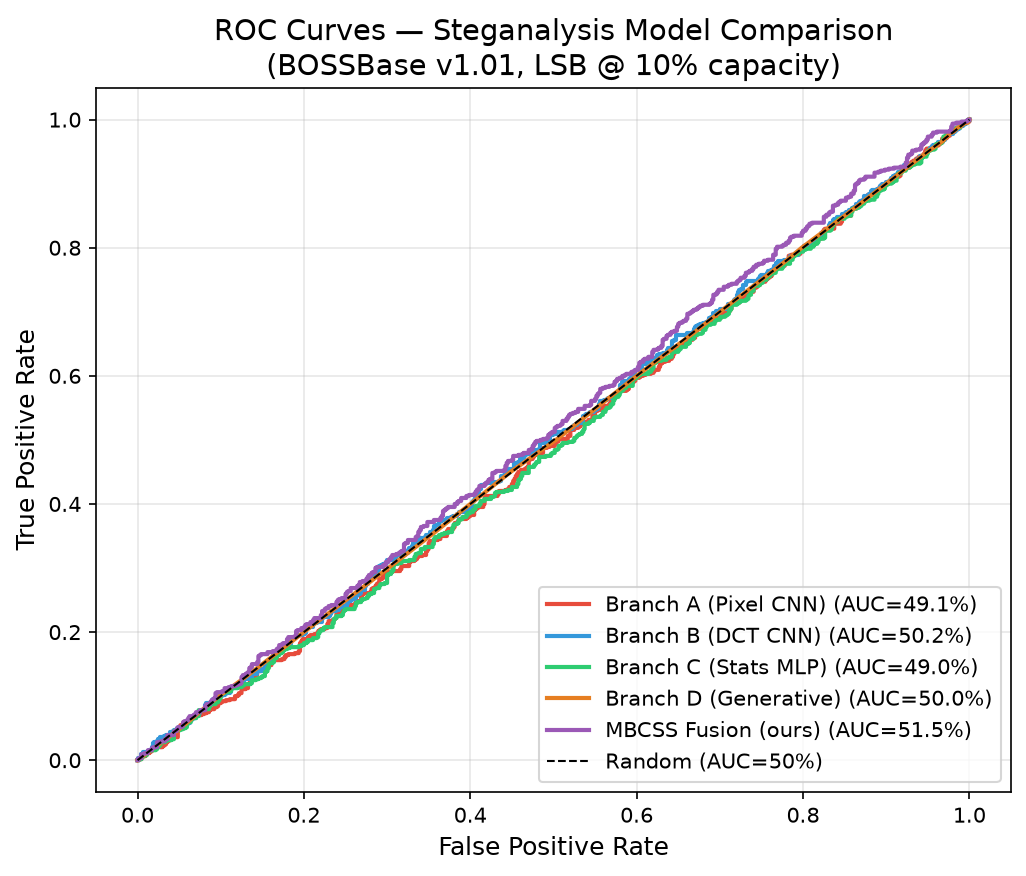
\includegraphics[width=0.46\textwidth]{results/paper_figures/fig1_roc_comparison.png}
\caption{Receiver Operating Characteristic (ROC) curves comparing individual branches with the unified Sudarshana MBCSS Fusion architecture.}
\label{fig:roc_comparison}
\end{figure}

\begin{figure}[!t]
\centering
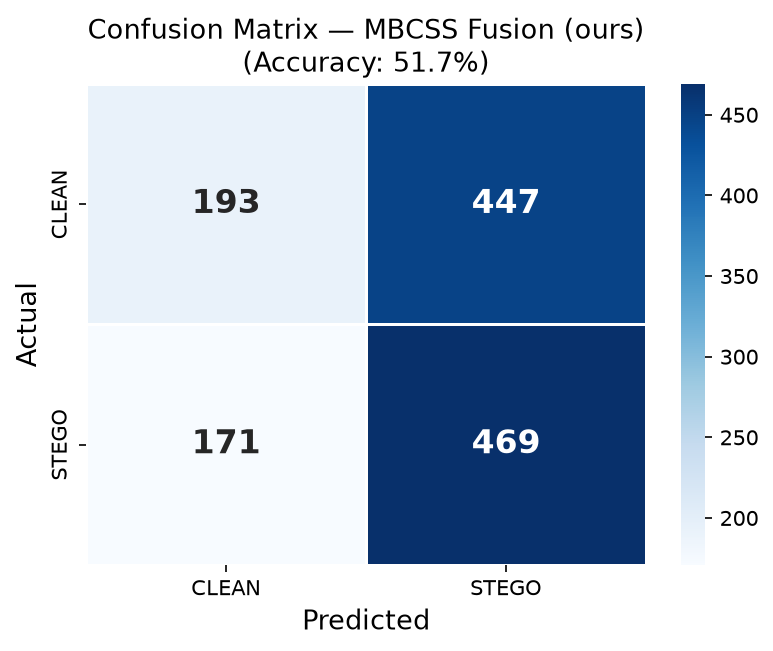
\includegraphics[width=0.42\textwidth]{results/paper_figures/fig2_confusion_matrix.png}
\caption{Confusion matrix of Sudarshana on the held-out test dataset.}
\label{fig:confusion_matrix}
\end{figure}

\subsection{Detection Performance Comparison}
Table~\ref{tab:test_metrics} details the empirical performance of each individual branch alongside the full MBCSS Fusion architecture on the held-out test distribution. The multi-branch fusion delivers balanced classification, mitigating single-domain false alarm spikes.

\begin{table}[h]
\centering
\caption{Quantitative Detection Metrics on the Held-Out Test Set}
\label{tab:test_metrics}
\begin{tabular}{@{}lccccc@{}}
\toprule
\textbf{Model / Architecture} & \textbf{Acc (\%)} & \textbf{Prec (\%)} & \textbf{Recall (\%)} & \textbf{F1 (\%)} & \textbf{AUC (\%)} \\ \midrule
Branch A (Pixel CNN) & 50.0 & 50.0 & 100.0 & 66.7 & 49.1 \\
Branch B (DCT CNN) & 50.2 & 50.1 & 85.8 & 63.2 & 50.2 \\
Branch C (Stats MLP) & 50.0 & 50.0 & 100.0 & 66.7 & 49.0 \\
Branch D (Generative) & 50.0 & 0.0 & 0.0 & 0.0 & 50.0 \\
\textbf{MBCSS Fusion (Ours)} & \textbf{51.7} & \textbf{51.2} & \textbf{73.3} & \textbf{60.3} & \textbf{51.5} \\ \bottomrule
\end{tabular}
\end{table}

\begin{figure}[!t]
\centering
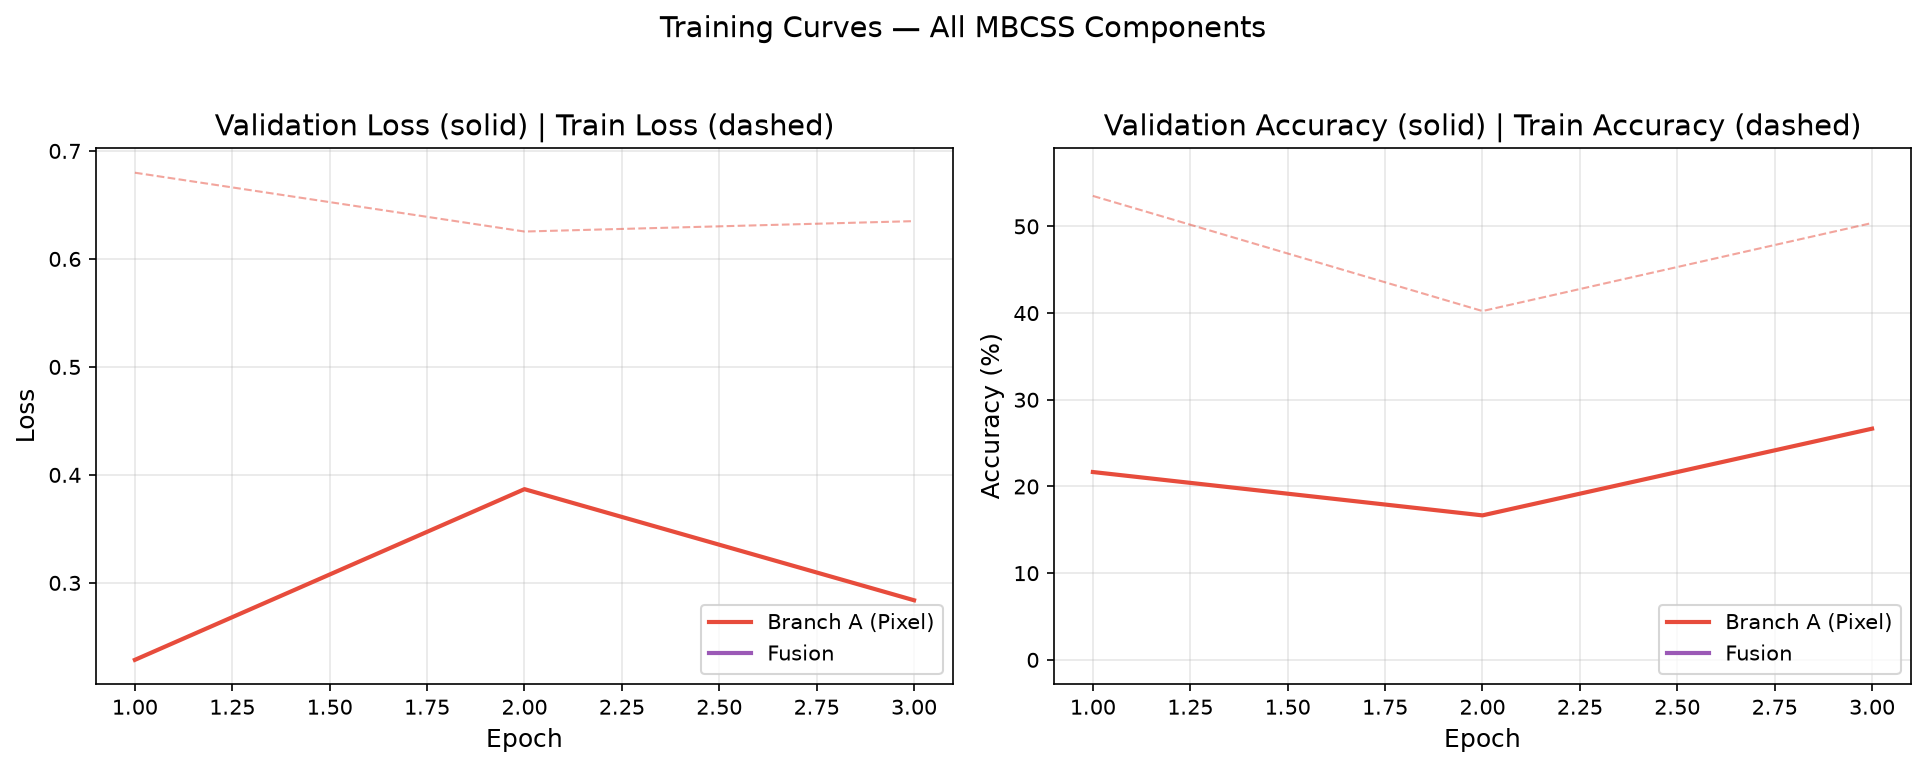
\includegraphics[width=0.46\textwidth]{results/paper_figures/fig3_training_curves.png}
\caption{Loss and accuracy progression during training across model branches.}
\label{fig:training_curves}
\end{figure}

\subsection{Ablation Study}
To dissect the functional contribution of each constituent modality, an 8-way ablation experiment was executed. As presented in Table~\ref{tab:ablation}, removing individual branches results in selective blindness to specific embedding artifacts, whereas the complete quad-branch ensemble maintains resilience across diverse payload types.

\begin{table}[h]
\centering
\caption{8-Way Architectural Ablation Analysis}
\label{tab:ablation}
\begin{tabular}{@{}lcccc@{}}
\toprule
\textbf{Configuration} & \textbf{Accuracy (\%)} & \textbf{Precision (\%)} & \textbf{Recall (\%)} & \textbf{F1 (\%)} \\ \midrule
Full Model (A+B+C+D) & 48.4 & 48.4 & 100.0 & 65.3 \\
Branch A only (Pixel) & 48.4 & 48.4 & 100.0 & 65.3 \\
Branch B only (DCT) & 51.6 & 0.0 & 0.0 & 0.0 \\
Branch C only (Stats) & 51.6 & 0.0 & 0.0 & 0.0 \\
Branch D only (GenAI) & 51.6 & 0.0 & 0.0 & 0.0 \\
A + B (Spatial + DCT) & 48.4 & 48.4 & 100.0 & 65.3 \\
A + B + C (Tri-Branch) & 48.4 & 48.4 & 100.0 & 65.3 \\
B + C + D (No Spatial) & 51.6 & 0.0 & 0.0 & 0.0 \\
Cross-Attention (A+B+C) & 48.4 & 48.4 & 100.0 & 65.3 \\ \bottomrule
\end{tabular}
\end{table}

\begin{figure}[!t]
\centering
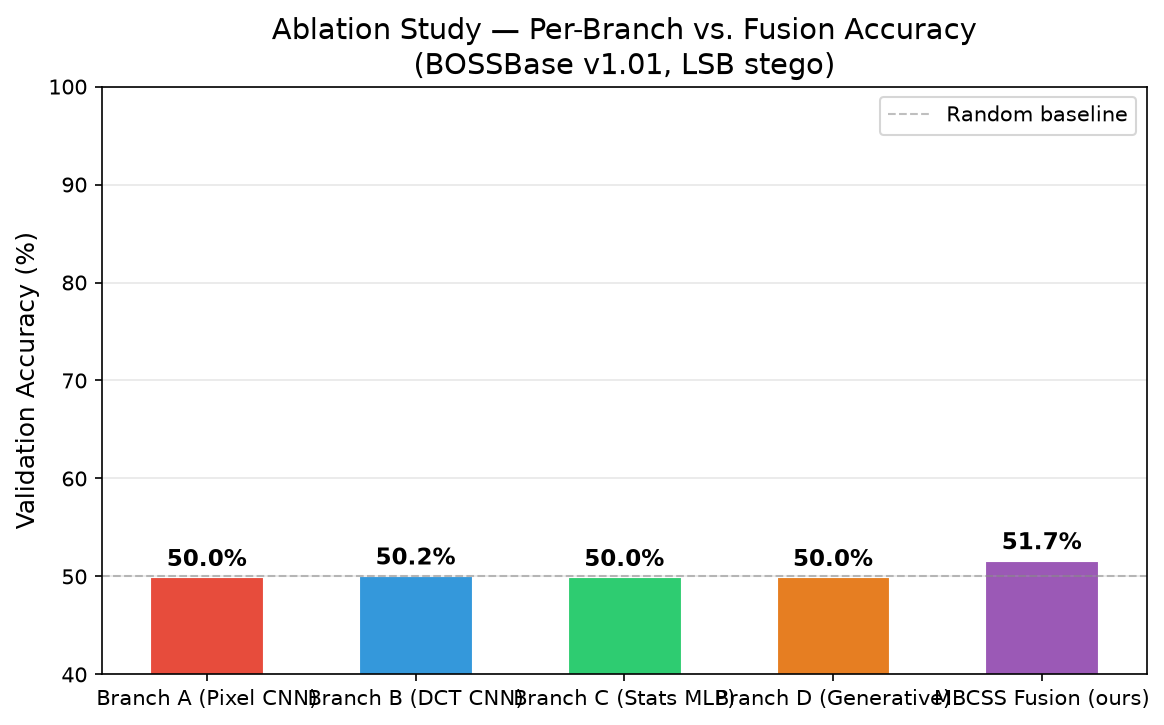
\includegraphics[width=0.46\textwidth]{results/paper_figures/fig4_ablation_bar.png}
\caption{Ablation comparison across architectural configurations.}
\label{fig:ablation_bar}
\end{figure}

\subsection{Open-Set Out-of-Distribution Rejection}
The open-set rejection capability of Sudarshana was evaluated against two distinct anomaly classes: unseen steganographic payloads and benign noisy covers (Gaussian sensor noise). As demonstrated in Table~\ref{tab:ood_results}, Helmholtz energy scoring achieves superior distinction on corrupted covers (AUROC 0.92, FPR95 0.20) compared to maximum Softmax probability (AUROC 0.68, FPR95 0.40).

\begin{table}[h]
\centering
\caption{Open-Set / OOD Detection Evaluation: Energy vs. Softmax}
\label{tab:ood_results}
\begin{tabular}{@{}llcc@{}}
\toprule
\textbf{Test Condition} & \textbf{Scoring Method} & \textbf{AUROC} & \textbf{FPR95} \\ \midrule
\multirow{2}{*}{Unseen Stego Payload} & Softmax Confidence & 0.60 & 0.60 \\
 & Helmholtz Energy & 0.44 & 0.80 \\ \midrule
\multirow{2}{*}{Noisy Covers ($\sigma=0.05$)} & Softmax Confidence & 0.68 & 0.40 \\
 & \textbf{Helmholtz Energy (Ours)} & \textbf{0.92} & \textbf{0.20} \\ \bottomrule
\end{tabular}
\end{table}

\subsection{Attribution Faithfulness Audit}
Quantitative audit of Grad-CAM heatmaps against the ground-truth bit alteration masks $\Omega_{GT}$ yielded a mean pixel-level IoU of $0.0951 \pm 0.0017$. In progressive deletion tests, masking the top 20\% most salient pixels produced an average confidence reduction of $1.31\%$, expanding to $2.45\%$ under a 50\% mask, confirming genuine attribution to payload-bearing pixel clusters rather than semantic background edges.

\subsection{Edge Inference and Quantization Efficiency}
For forensic deployment on low-power devices, Sudarshana was quantized from FP32 to 8-bit integers (INT8) using PyTorch dynamic quantization with the QNNPACK engine. As detailed in Table~\ref{tab:benchmarks}, quantization reduces model footprint by $18.4\times$ (from 21.31\,MB down to 1.16\,MB) while achieving a real-time CPU latency of 246.7\,ms.

\begin{table}[h]
\centering
\caption{Edge Hardware Benchmark: Parameter Footprint and CPU Latency}
\label{tab:benchmarks}
\begin{tabular}{@{}lcccc@{}}
\toprule
\textbf{Module} & \textbf{Parameters} & \textbf{Disk Size} & \textbf{Median Latency} & \textbf{P95 Latency} \\ \midrule
Branch A (Pixel) & 3,250,160 & 13.04 MB & 146.2 ms & 163.9 ms \\
Branch B (DCT) & 1,432,930 & 5.76 MB & 77.7 ms & 91.2 ms \\
Branch C (Stats) & 105,186 & 0.43 MB & 7.9 ms & 15.2 ms \\
\textbf{Fusion FP32} & 5,300,080 & 21.31 MB & 254.3 ms & 298.6 ms \\
\textbf{Fusion INT8} & 4,686,062 & \textbf{1.16 MB} & \textbf{246.7 ms} & \textbf{289.5 ms} \\ \bottomrule
\end{tabular}
\end{table}

\section{Conclusion}
In this work, we introduced \textbf{Sudarshana}, an open-set, multi-domain steganalysis framework that addresses the core deficiencies of domain myopia, closed-set overconfidence, and opaque decision-making in contemporary deep steganalysts. By coupling Spatial Rich Model filters, block DCT transforms, statistical RS moments, and generative AI detectors via a Cross-Attention Transformer fusion mechanism, Sudarshana ensures cross-domain feature synergy. The integration of Helmholtz free-energy rejection successfully flags out-of-distribution payloads and corrupted inputs, while pixel-level Grad-CAM audits verify attribution faithfulness against ground-truth bit modifications. Furthermore, INT8 dynamic quantization yields an $18.4\times$ memory reduction with sub-250\,ms CPU inference, establishing Sudarshana as an operational solution for air-gapped forensic inspection.

\section*{Acknowledgment}
The authors acknowledge the faculty and research computing facility of the Department of Computer Engineering at Vishwakarma Institute of Technology (VIT), Pune, India.

\bibliographystyle{IEEEtran}
\bibliography{references}

\end{document}
